\documentclass[]{book}
\usepackage{lmodern}
\usepackage{amssymb,amsmath}
\usepackage{ifxetex,ifluatex}
\usepackage{fixltx2e} % provides \textsubscript
\ifnum 0\ifxetex 1\fi\ifluatex 1\fi=0 % if pdftex
  \usepackage[T1]{fontenc}
  \usepackage[utf8]{inputenc}
\else % if luatex or xelatex
  \ifxetex
    \usepackage{mathspec}
  \else
    \usepackage{fontspec}
  \fi
  \defaultfontfeatures{Ligatures=TeX,Scale=MatchLowercase}
\fi
% use upquote if available, for straight quotes in verbatim environments
\IfFileExists{upquote.sty}{\usepackage{upquote}}{}
% use microtype if available
\IfFileExists{microtype.sty}{%
\usepackage{microtype}
\UseMicrotypeSet[protrusion]{basicmath} % disable protrusion for tt fonts
}{}
\usepackage[margin=1in]{geometry}
\usepackage{hyperref}
\hypersetup{unicode=true,
            pdftitle={Supplement to Shiny in Production},
            pdfborder={0 0 0},
            breaklinks=true}
\urlstyle{same}  % don't use monospace font for urls
\usepackage{natbib}
\bibliographystyle{plainnat}
\usepackage{color}
\usepackage{fancyvrb}
\newcommand{\VerbBar}{|}
\newcommand{\VERB}{\Verb[commandchars=\\\{\}]}
\DefineVerbatimEnvironment{Highlighting}{Verbatim}{commandchars=\\\{\}}
% Add ',fontsize=\small' for more characters per line
\usepackage{framed}
\definecolor{shadecolor}{RGB}{248,248,248}
\newenvironment{Shaded}{\begin{snugshade}}{\end{snugshade}}
\newcommand{\AlertTok}[1]{\textcolor[rgb]{0.94,0.16,0.16}{#1}}
\newcommand{\AnnotationTok}[1]{\textcolor[rgb]{0.56,0.35,0.01}{\textbf{\textit{#1}}}}
\newcommand{\AttributeTok}[1]{\textcolor[rgb]{0.77,0.63,0.00}{#1}}
\newcommand{\BaseNTok}[1]{\textcolor[rgb]{0.00,0.00,0.81}{#1}}
\newcommand{\BuiltInTok}[1]{#1}
\newcommand{\CharTok}[1]{\textcolor[rgb]{0.31,0.60,0.02}{#1}}
\newcommand{\CommentTok}[1]{\textcolor[rgb]{0.56,0.35,0.01}{\textit{#1}}}
\newcommand{\CommentVarTok}[1]{\textcolor[rgb]{0.56,0.35,0.01}{\textbf{\textit{#1}}}}
\newcommand{\ConstantTok}[1]{\textcolor[rgb]{0.00,0.00,0.00}{#1}}
\newcommand{\ControlFlowTok}[1]{\textcolor[rgb]{0.13,0.29,0.53}{\textbf{#1}}}
\newcommand{\DataTypeTok}[1]{\textcolor[rgb]{0.13,0.29,0.53}{#1}}
\newcommand{\DecValTok}[1]{\textcolor[rgb]{0.00,0.00,0.81}{#1}}
\newcommand{\DocumentationTok}[1]{\textcolor[rgb]{0.56,0.35,0.01}{\textbf{\textit{#1}}}}
\newcommand{\ErrorTok}[1]{\textcolor[rgb]{0.64,0.00,0.00}{\textbf{#1}}}
\newcommand{\ExtensionTok}[1]{#1}
\newcommand{\FloatTok}[1]{\textcolor[rgb]{0.00,0.00,0.81}{#1}}
\newcommand{\FunctionTok}[1]{\textcolor[rgb]{0.00,0.00,0.00}{#1}}
\newcommand{\ImportTok}[1]{#1}
\newcommand{\InformationTok}[1]{\textcolor[rgb]{0.56,0.35,0.01}{\textbf{\textit{#1}}}}
\newcommand{\KeywordTok}[1]{\textcolor[rgb]{0.13,0.29,0.53}{\textbf{#1}}}
\newcommand{\NormalTok}[1]{#1}
\newcommand{\OperatorTok}[1]{\textcolor[rgb]{0.81,0.36,0.00}{\textbf{#1}}}
\newcommand{\OtherTok}[1]{\textcolor[rgb]{0.56,0.35,0.01}{#1}}
\newcommand{\PreprocessorTok}[1]{\textcolor[rgb]{0.56,0.35,0.01}{\textit{#1}}}
\newcommand{\RegionMarkerTok}[1]{#1}
\newcommand{\SpecialCharTok}[1]{\textcolor[rgb]{0.00,0.00,0.00}{#1}}
\newcommand{\SpecialStringTok}[1]{\textcolor[rgb]{0.31,0.60,0.02}{#1}}
\newcommand{\StringTok}[1]{\textcolor[rgb]{0.31,0.60,0.02}{#1}}
\newcommand{\VariableTok}[1]{\textcolor[rgb]{0.00,0.00,0.00}{#1}}
\newcommand{\VerbatimStringTok}[1]{\textcolor[rgb]{0.31,0.60,0.02}{#1}}
\newcommand{\WarningTok}[1]{\textcolor[rgb]{0.56,0.35,0.01}{\textbf{\textit{#1}}}}
\usepackage{longtable,booktabs}
\usepackage{graphicx,grffile}
\makeatletter
\def\maxwidth{\ifdim\Gin@nat@width>\linewidth\linewidth\else\Gin@nat@width\fi}
\def\maxheight{\ifdim\Gin@nat@height>\textheight\textheight\else\Gin@nat@height\fi}
\makeatother
% Scale images if necessary, so that they will not overflow the page
% margins by default, and it is still possible to overwrite the defaults
% using explicit options in \includegraphics[width, height, ...]{}
\setkeys{Gin}{width=\maxwidth,height=\maxheight,keepaspectratio}
\IfFileExists{parskip.sty}{%
\usepackage{parskip}
}{% else
\setlength{\parindent}{0pt}
\setlength{\parskip}{6pt plus 2pt minus 1pt}
}
\setlength{\emergencystretch}{3em}  % prevent overfull lines
\providecommand{\tightlist}{%
  \setlength{\itemsep}{0pt}\setlength{\parskip}{0pt}}
\setcounter{secnumdepth}{5}
% Redefines (sub)paragraphs to behave more like sections
\ifx\paragraph\undefined\else
\let\oldparagraph\paragraph
\renewcommand{\paragraph}[1]{\oldparagraph{#1}\mbox{}}
\fi
\ifx\subparagraph\undefined\else
\let\oldsubparagraph\subparagraph
\renewcommand{\subparagraph}[1]{\oldsubparagraph{#1}\mbox{}}
\fi

%%% Use protect on footnotes to avoid problems with footnotes in titles
\let\rmarkdownfootnote\footnote%
\def\footnote{\protect\rmarkdownfootnote}

%%% Change title format to be more compact
\usepackage{titling}

% Create subtitle command for use in maketitle
\newcommand{\subtitle}[1]{
  \posttitle{
    \begin{center}\large#1\end{center}
    }
}

\setlength{\droptitle}{-2em}

  \title{Supplement to Shiny in Production}
    \pretitle{\vspace{\droptitle}\centering\huge}
  \posttitle{\par}
    \author{}
    \preauthor{}\postauthor{}
      \predate{\centering\large\emph}
  \postdate{\par}
    \date{2019-01-05}

\usepackage{booktabs}

\usepackage{amsthm}
\newtheorem{theorem}{Theorem}[chapter]
\newtheorem{lemma}{Lemma}[chapter]
\theoremstyle{definition}
\newtheorem{definition}{Definition}[chapter]
\newtheorem{corollary}{Corollary}[chapter]
\newtheorem{proposition}{Proposition}[chapter]
\theoremstyle{definition}
\newtheorem{example}{Example}[chapter]
\theoremstyle{definition}
\newtheorem{exercise}{Exercise}[chapter]
\theoremstyle{remark}
\newtheorem*{remark}{Remark}
\newtheorem*{solution}{Solution}
\begin{document}
\maketitle

{
\setcounter{tocdepth}{1}
\tableofcontents
}
\hypertarget{shiny-in-production-workshop-rstudio-conf-2019}{%
\chapter{Shiny in Production Workshop @ RStudio Conf
2019}\label{shiny-in-production-workshop-rstudio-conf-2019}}

This document is full of supplemental resources and content from the
Shiny in Production Workshop delievered at rstudio::conf 2019.

The \textbf{bookdown} package can be installed from CRAN or Github:

\begin{Shaded}
\begin{Highlighting}[]
\KeywordTok{install.packages}\NormalTok{(}\StringTok{"bookdown"}\NormalTok{)}
\CommentTok{# or the development version}
\CommentTok{# devtools::install_github("rstudio/bookdown")}
\end{Highlighting}
\end{Shaded}

\hypertarget{course-intro}{%
\chapter{Introduction to Shiny in Production}\label{course-intro}}

\hypertarget{why-are-we-here}{%
\section{Why are we here?}\label{why-are-we-here}}

\begin{quote}
Shiny applications are being deployed in high-value, customer-facing,
and/or enterprise-wide scenarios. Unfortunately, they are often being
done without the benefit of best practices. This workshop will help you
and/or your IT colleagues who support your data scientists learn how to
accelerate a successful Shiny application deployment in production
scenarios.
\end{quote}

Over the past year, software developers at RStudio have been working
hard to dispel rumors that Shiny ``isn't ready and can't run in
production''. They've built a bunch of cool new tools that are useful in
preparing applications for production and understanding how to configure
and scale them for optimized performance and user experience.

This workshop will cover all these new tools for shiny development as
well as the equally important logistical pieces of a production story:

\begin{itemize}
\tightlist
\item
  What does production infrastructure and tooling look like for Shiny
  apps?
\item
  How do we get Shiny apps from development into production?
\item
  How are Shiny apps maintained production?
\end{itemize}

\begin{quote}
When developers begin to think of infrastructure as part of their
application, stability and performance become normative. - Jeff Geerling
``Ansible for DevOps''
\end{quote}

\hypertarget{can-shiny-be-used-in-production}{%
\subsection{Can Shiny be used in
production?}\label{can-shiny-be-used-in-production}}

\hypertarget{objectives}{%
\subsection{Objectives}\label{objectives}}

\hypertarget{understand-the-importance-of-incremental-changes-and-testing}{%
\subsubsection{Understand the importance of incremental changes and
testing}\label{understand-the-importance-of-incremental-changes-and-testing}}

\begin{itemize}
\tightlist
\item
  Version control
\item
  Tests for package upgrades
\item
  Use of separate environments for staging and production
\item
  Incorporating automated testing into a development workflow:
  \texttt{shinytest}
\end{itemize}

\hypertarget{data-product-tradeoffs}{%
\subsubsection{Data product tradeoffs}\label{data-product-tradeoffs}}

\begin{itemize}
\tightlist
\item
  What are the advantages to using Shiny vs Plumber vs R Markdown
\item
  What is the difference between a stateless Plumber API and a Shiny
  Session?
\end{itemize}

\hypertarget{development-vs.production-environment-considerations}{%
\subsubsection{Development vs.~Production environment
considerations}\label{development-vs.production-environment-considerations}}

\begin{itemize}
\tightlist
\item
  Defining a data model

  \begin{itemize}
  \tightlist
  \item
    Working with databases
  \end{itemize}
\item
  Tools for understanding application performance

  \begin{itemize}
  \tightlist
  \item
    \texttt{shinyloadtest}
  \item
    \texttt{profvis}
  \end{itemize}
\item
  Tools for improving application performance

  \begin{itemize}
  \tightlist
  \item
    Plot caching
  \item
    Synchronous vs asynchronous paradigms: \texttt{async}
  \end{itemize}
\end{itemize}

\hypertarget{deployment-architecture-and-tools}{%
\subsubsection{Deployment architecture and
tools}\label{deployment-architecture-and-tools}}

\begin{itemize}
\tightlist
\item
  Introduction to analytic infrastructure
\item
  Configuration management
\item
  Resources for scaling horizontally
\end{itemize}

\hypertarget{outline}{%
\section{Outline}\label{outline}}

\hypertarget{workshop-infrastructure}{%
\section{Workshop Infrastructure}\label{workshop-infrastructure}}

\begin{itemize}
\tightlist
\item
  RStudio Connect
\item
  PostgreSQL
\end{itemize}

Instructions for accessing the classroom environment are available in
the workshop slide deck.

\hypertarget{app-intro}{%
\chapter{Introduction to the Application}\label{app-intro}}

\hypertarget{every-application-has-an-origin-story}{%
\section{Every Application has an Origin
Story}\label{every-application-has-an-origin-story}}

Data Scientists at RStudio University have discovered that there are
trackable traits and behaviors students engage in that have been
predictive of the desired 4-year graduation track.

They have built a shiny application that can be used by the very
data-savvy advisors at this illustrious institution to identify students
in need of guidance and show them the top behavioral factors driving
individual predictions coming out of the model.

The POC was a smashing success - but now \emph{the advisors actually
want to use this thing for real}.

\begin{itemize}
\tightlist
\item
  We've developed a nice app
\item
  We want to put it into production
\item
  We want confidence that it will perform well in production, both now
  and in the future
\end{itemize}

\hypertarget{activity-explore-the-application}{%
\subsection{Activity: Explore the
Application}\label{activity-explore-the-application}}

Open the POC Application Run the Application Explore the Application
code

\begin{enumerate}
\def\labelenumi{\arabic{enumi}.}
\tightlist
\item
  Are there any parts of the application code that don't make sense?
\item
  Brainstorm: what qualifies as production?
\item
  Brainstorm: 5 things to consider when bringing this application into
  production.
\end{enumerate}

What are our application requirements? - Who does this app serve? - What
kind of utilization do we expect? - Expected concurrent usage, can we
handle peaks/spikes? - What happens if we under budget? Do we have
strategies for scaling up? - What happens if we over budget? Do we have
strategies for scaling down? - How will this all be monitored?

\begin{center}\rule{0.5\linewidth}{\linethickness}\end{center}

Discussion

\begin{itemize}
\tightlist
\item
  Is this app ready for production?
\item
  What insights would be useful to have before taking this app into
  production?
\item
  What tools currently exist that would help us run tests to gain these
  insights?
\end{itemize}

\textbf{Create a checklist for taking this (any?) application into
production}

\begin{itemize}
\tightlist
\item
  What is your current process for taking applications into production?
\end{itemize}

\hypertarget{is-shiny-the-right-medium-data-produt-for-this-project}{%
\subsection{Is Shiny the right medium (data produt) for this
project?}\label{is-shiny-the-right-medium-data-produt-for-this-project}}

\begin{itemize}
\tightlist
\item
  Alternative Architectures (later chapter)
\end{itemize}

\hypertarget{understanding-the-app-reactlog}{%
\section{\texorpdfstring{Understanding the App:
\texttt{reactlog}}{Understanding the App: reactlog}}\label{understanding-the-app-reactlog}}

\begin{verbatim}
library(shinyreactlog)
options(shiny.reactlog = True)
runApp()
\end{verbatim}

\href{https://shiny.rstudio.com/reference/shiny/0.14/showReactLog.html}{React
Log Visualizer Reference}

\begin{quote}
For security and performance reasons, do not enable shiny.reactlog in
production environments. When the option is enabled, it's possible for
any user of your app to see at least some of the source code of your
reactive expressions and observers.
\end{quote}

\hypertarget{checklist-for-taking-applications-into-production}{%
\section{Checklist for Taking Applications into
Production}\label{checklist-for-taking-applications-into-production}}

A high-level Checklist to build off of:

\begin{itemize}
\tightlist
\item
  {[} {]} Tests
\item
  {[} {]} Performance Optimization
\item
  {[} {]} Environment (Package) Management
\item
  {[} {]} Data Access
\item
  {[} {]} Deployment Hand Off
\item
  {[} {]} Scaling
\item
  {[} {]} Monitoring
\end{itemize}

\hypertarget{application-testing-shinytest}{%
\chapter{\texorpdfstring{Application Testing:
\texttt{shinytest}}{Application Testing: shinytest}}\label{application-testing-shinytest}}

{[}From the Webinar{]} - You've developed a nice app - You've put it in
production - You want to be confident that it will keep running in the
future

\textbf{Things that can change/break a Shiny application} - Modifying
code - Upgrading the \texttt{shiny} package - Upgrading other packages -
Upgrading R - External data source changes or fails

\hypertarget{testing-options}{%
\subsection{Testing Options}\label{testing-options}}

\begin{itemize}
\tightlist
\item
  Manual testing

  \begin{itemize}
  \tightlist
  \item
    time intensive
  \item
    inconsistent
  \end{itemize}
\item
  Automated testing (hard)

  \begin{itemize}
  \tightlist
  \item
    web browser
  \item
    simulated user interactions
  \item
    tests for graphical elements
  \end{itemize}
\end{itemize}

Shinytest:
\url{https://github.com/rstudio/webinars/blob/master/48-shinytest/shinytest.pdf}

{[}demo on the Geyser app{]}

\hypertarget{from-the-blog}{%
\section{From the Blog}\label{from-the-blog}}

\href{https://resources.rstudio.com/rstudio-blog/shinytest-automated-testing-for-shiny-apps}{Blog}

\texttt{shinytest} is a package (available on CRAN) to perform automated
testing for Shiny apps.

\begin{itemize}
\tightlist
\item
  Record Shiny tests
\item
  Run and troubleshoot Shiny tests
\end{itemize}

Support for \texttt{shinytest} is available in RStudio v1.2 preview

\hypertarget{installation}{%
\section{Installation}\label{installation}}

`install.packages(``shinytest'')

\textbf{Note:} When running \texttt{shinytest} for the first time, you
may be prompted by the RStudio IDE or package warning messages to
install some dependencies. \texttt{shinytest} requires a headless web
browser (PhantomJS) to record and run tests. - To install it, run
shinytest::installDependencies() - If it is installed, make sure the
phantomjs executable can be found via the PATH variable.

\hypertarget{record-tests}{%
\section{Record Tests}\label{record-tests}}

\begin{itemize}
\tightlist
\item
  Run \texttt{recordTest()} to launch the app in a test recorder.
\item
  Create the tests by interacting with the application - this will allow
  the recorder to snapshot the application state at various points.
\item
  Quit the test recorder. This action will trigger the following events:

  \begin{itemize}
  \tightlist
  \item
    The test script will be saved as a .R file in a subdirectory of the
    application named \texttt{tests/}.
  \item
    If you are running in the RStudio IDE, it will automatically open
    this file in the editor.
  \item
    The test script will be run, and the snapshots will be saved in a
    subdirectory of the \texttt{tests/} directory.
  \end{itemize}
\end{itemize}

To record tests from \texttt{R}, run the following:

\begin{verbatim}
library(shinytest)

recordTest("path/to/the/app")   #Replace with the correct path
\end{verbatim}

To record tests from RStudio v1.2, when an application file (app.R,
server.R, ui.R or global.R) is open in the editor, a button labeled
\emph{Run App} will appear at the top of the editor pane. Click on the
small black triangle next to this button to reveal the menu of extended
options.

\begin{figure}
\centering
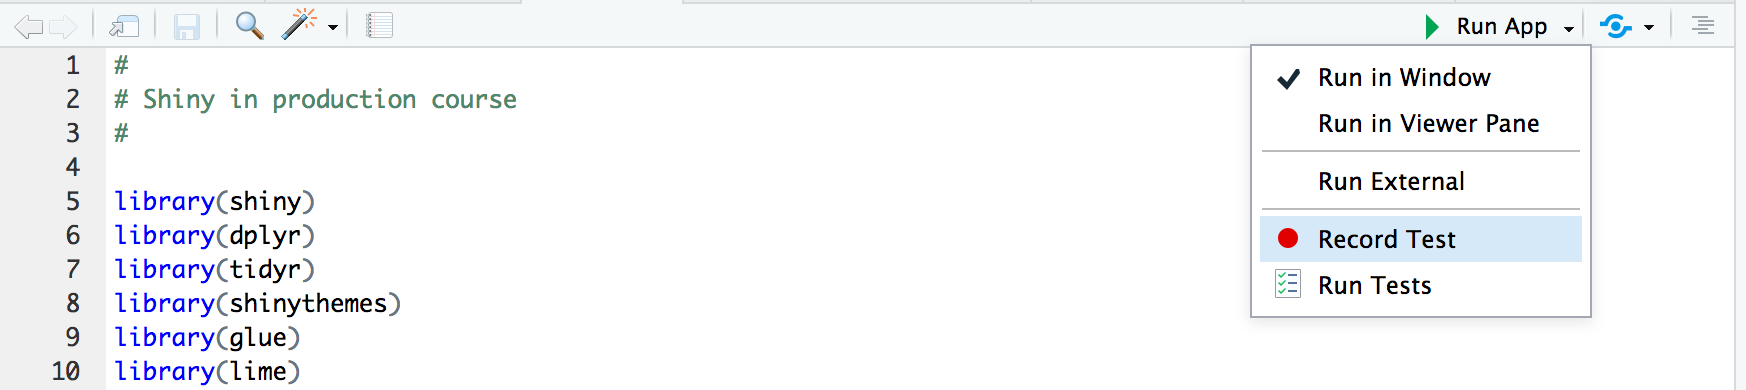
\includegraphics{imgs/testing/record_test_button.png}
\caption{Record Test Button}
\end{figure}

This launches the Shiny application to be tested in a separate R
process. We'll refer to this as the \textbf{target app}. At the same
time, the current R process lauches a special Shiny application which
displays the target app in an iframe along with some controls. We'll
refer to this as the \textbf{recorder app}. You should see something
like this:

\begin{figure}
\centering
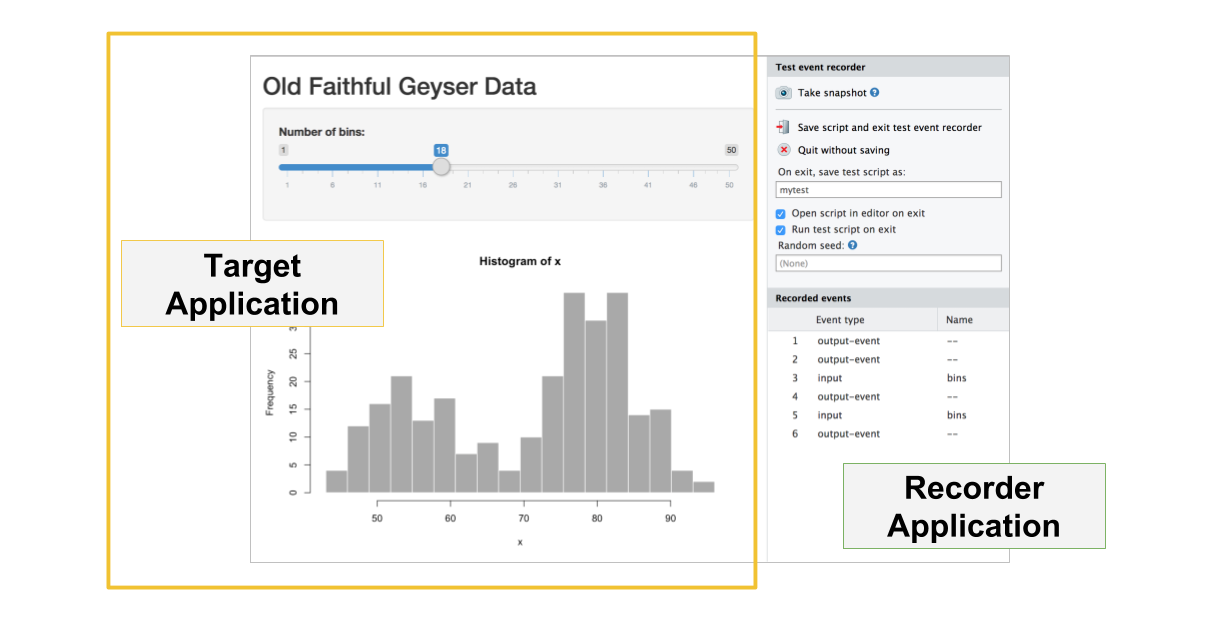
\includegraphics{imgs/testing/recorder_and_target.png}
\caption{Target and Recorder App iframe}
\end{figure}

The panel on the right displays some controls for the test recorder, as
well as a list of \textbf{recorded events}. As you interact with the
target app, you will see those interactions appear in the recorded
events list.

For testing a Shiny application, interacting with the inputs is only one
part of the equation. It's also necessary to check that the application
produces the correct outputs. This is accomplished by taking
\textbf{snapshots} of the application's state.

To take a snapshot of the application's state, click the \emph{Take
snapshot} button on the recorder app. This will record all input values,
output values, and exported values.

\hypertarget{running-tests}{%
\section{Running Tests}\label{running-tests}}

When you quit the test recorder, it will automatically run the test
script. There are three separate components involved in running tests:

\begin{enumerate}
\def\labelenumi{\arabic{enumi}.}
\tightlist
\item
  First is the \textbf{test driver}. This is the R process that
  coordiates the testing and controls the web browser. When working on
  creating tests interactively, this is the R process that you use.
\item
  Next is the \textbf{Shiny process}, also known as the \textbf{server}.
  This is the R process that runs the target Shiny application.
\item
  Finally, there is the \textbf{web browser}, also known as the
  \textbf{client}, which connects to the server. This is a headless web
  browser - one which renders the web page internally, but doesn't
  display the content to the screen (PhantomJS).
\end{enumerate}

So, when you exit the test recorder, it will by default automatically
run the test script and print something like this:

\begin{verbatim}
Saved test code to /path/to/app/tests/mytest.R
Running mytest.R 
====== Comparing mytest ...
  No existing snapshots at mytest-expected/. This is a first run of tests.

Updating baseline snapshot at tests/mytest-expected
Renaming tests/mytest-current
      => tests/mytest-expected.
\end{verbatim}

This is the result of running \texttt{testApp()}, which can also be
manually run by providing the desired application and test like this:

\texttt{testApp("exampleApp",\ "mytest")}

The built-in integreation with RStudio v1.2 provides \texttt{Run\ Tests}
as a drop down menu option in your Shiny app source file (see it located
under the \emph{Record Test} option in the screenshot above).

\hypertarget{subsequent-test-runs}{%
\section{Subsequent Test Runs}\label{subsequent-test-runs}}

After the initial test run, you can continue to run the tests to check
for changes in application behavior.

If there are any differences between current and expected results, the
test output will look something like this:

\begin{verbatim}
Running mytest.R 
====== Comparing mytest ...
  Differences detected between mytest-current/ and mytest-expected/:

    Name         Status      
    001.json  != Files differ
    001.png   != Files differ
Would you like to view the differences between expected and current results [y/n]? 
\end{verbatim}

To view failed tests in the RStudio IDE, go to the \emph{Build tab} and
make sure the \emph{issues toggle} is selected:

\begin{figure}
\centering
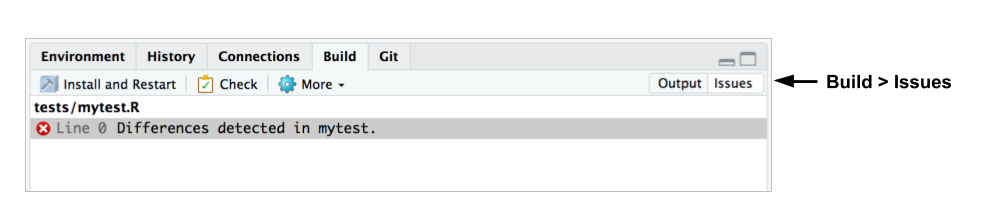
\includegraphics{imgs/testing/failed_tests.png}
\caption{View Failed Tests}
\end{figure}

For each test with different results, you can see the differences
between the expected and current results.

\hypertarget{testing-code}{%
\section{Testing Code}\label{testing-code}}

The \texttt{shinytest} package was created for testing Shiny
applications on the interaction-level. To test Shiny code and functions,
we suggest using the \texttt{testthat} package.

\href{http://testthat.r-lib.org/}{Info}
\href{https://github.com/r-lib/testthat}{GitHub}

Learn about testing and how to setup test workflow and structure:
\href{http://r-pkgs.had.co.nz/tests.html}{R packages by Hadley Wickham}

\hypertarget{profiling-the-most-important-thing}{%
\chapter{Profiling: ``The most important
thing''}\label{profiling-the-most-important-thing}}

\hypertarget{profivs}{%
\section{\texorpdfstring{\texttt{profivs}}{profivs}}\label{profivs}}

\href{https://github.com/rstudio/webinars/blob/master/26-Profiling/Profiling.pdf}{Webinar
Slides}

\hypertarget{deployment-rstudio-connect}{%
\chapter{Deployment: RStudio Connect}\label{deployment-rstudio-connect}}

\hypertarget{rstudio-connect}{%
\section{RStudio Connect}\label{rstudio-connect}}

\hypertarget{packrat}{%
\section{Packrat}\label{packrat}}

\hypertarget{connecting-to-data-in-production}{%
\chapter{Connecting to Data in
Production}\label{connecting-to-data-in-production}}

\hypertarget{databases}{%
\section{Databases}\label{databases}}

\hypertarget{config}{%
\section{\texorpdfstring{\texttt{config}}{config}}\label{config}}

\hypertarget{load-testing}{%
\chapter{Load Testing}\label{load-testing}}

\hypertarget{shinyloadtest}{%
\section{\texorpdfstring{\texttt{shinyloadtest}}{shinyloadtest}}\label{shinyloadtest}}

\href{https://github.com/rstudio/webinars/blob/master/63-shinyloadtest/slides.pdf}{Webinar
Slides}

\hypertarget{plot-caching}{%
\chapter{Plot Caching}\label{plot-caching}}

\hypertarget{scaling}{%
\chapter{Scaling}\label{scaling}}

\hypertarget{application-scaling-101}{%
\section{Application Scaling 101}\label{application-scaling-101}}

\begin{itemize}
\tightlist
\item
  cooking/ kitchen metaphor
\end{itemize}

\hypertarget{rstudio-connect-performance-settings}{%
\section{RStudio Connect Performance
Settings}\label{rstudio-connect-performance-settings}}

\hypertarget{devops-philosophy-tooling}{%
\chapter{DevOps Philosophy \& Tooling}\label{devops-philosophy-tooling}}

\hypertarget{devops-vocab-101}{%
\section{DevOps Vocab 101}\label{devops-vocab-101}}

\hypertarget{design-and-management-of-analytic-infrastructure-alternative-architectures}{%
\section{Design and Management of Analytic Infrastructure (alternative
architectures)}\label{design-and-management-of-analytic-infrastructure-alternative-architectures}}

\hypertarget{programatic-deployment-into-rstudio-connect}{%
\section{Programatic Deployment into RStudio
Connect}\label{programatic-deployment-into-rstudio-connect}}

\hypertarget{production-case-studies}{%
\chapter{Production Case Studies}\label{production-case-studies}}

\hypertarget{case-study-a-devtestprod}{%
\section{Case Study A: Dev/Test/Prod}\label{case-study-a-devtestprod}}

\hypertarget{case-study-b-ci-git-chef}{%
\section{Case Study B: CI, Git, Chef}\label{case-study-b-ci-git-chef}}

\hypertarget{case-study-c-docker}{%
\section{Case Study C: Docker}\label{case-study-c-docker}}

\hypertarget{alternatives-to-shiny}{%
\chapter{Alternatives to Shiny}\label{alternatives-to-shiny}}

\hypertarget{plumber}{%
\section{Plumber}\label{plumber}}

\hypertarget{r-markdown}{%
\section{R Markdown}\label{r-markdown}}

\hypertarget{shiny-async}{%
\chapter{Shiny Async}\label{shiny-async}}

\href{https://github.com/rstudio/webinars/blob/master/56-scaling-shiny-apps/Scaling\%20Shiny\%20apps\%20with\%20async\%20programming.pdf}{Webinar
Slides}


\end{document}
